\documentclass[11pt,a4paper]{article}
\usepackage[T1]{fontenc}
\usepackage[margin=2.3cm]{geometry}
\usepackage{amsmath,amssymb}
\usepackage{graphicx}
\usepackage[dvipsnames]{xcolor}
\usepackage{enumitem}
\usepackage[colorlinks=true,linkcolor=blue,urlcolor=blue]{hyperref}
\setlength{\parskip}{0.6em}
\setlength{\parindent}{0pt}
\begin{document}

\begin{center}{\LARGE\bfseries openpathplanner}\\[0.4em]{\large Plan routes for a warehouse robot with A* and RRT, in three sessions.}\\[0.2em]\small PAN IIT OSS explainer \textbullet{} higher secondary to advanced undergraduate (levels 4-6)\end{center}

\section*{Why this exists}
Every warehouse robot, delivery robot and autonomous vehicle must decide how to get from here to there without hitting anything. This explainer shows the mathematics behind that decision with graph search and random sampling, so you can build it yourself.

\section*{The end goal}
Plan routes for a warehouse robot with A* and RRT. The end goal is route planning for a warehouse robot with A* and RRT, as used in path planning and obstacle avoidance for autonomous machines. The models are simplified teaching models and are not for controlling real robots or vehicles.

\section*{How the three sessions build up}
\begin{enumerate}[nosep]
\item \textbf{Session 1: The shortest path is not the straight line} (Level 1, conceptual interactive model, 60 min).
\item \textbf{Session 2: Graphs, Dijkstra and A*} (Level 2, mathematical engineering model, 80 min).
\item \textbf{Session 3: Continuous space: RRT, RRT* and validation} (Level 3, simulation and validation, 90 min).
\end{enumerate}

\section{Session 1: The shortest path is not the straight line}

\subsection*{A. Real-world problem}
A warehouse robot at the left of the floor must reach a shelf at the right. A long wall with one door stands between them. The straight line from robot to shelf runs through the wall, so the robot must walk to the door and back. How long is the real route, and how can a program find it without trying every possible walk? This is a simplified teaching model, not software for controlling a real robot.

\subsection*{B. Concept and theory}
We cut the floor into square cells. Each cell is free or blocked. The robot moves one cell at a time up, down, left or right, and every move costs one step. Breadth-first search (BFS) explores the floor in rings: first all cells one step from the robot, then all cells two steps away, and so on. The first time a ring touches the shelf, the number of the ring is the fewest possible steps. For cells dx columns and dy rows apart, the straight-line distance is sqrt(dx\textasciicircum{}2 + dy\textasciicircum{}2), but on an empty floor the 4-move route needs dx + dy steps, and any wall can only make the route longer, never shorter.

\begin{itemize}[nosep]
\item dx, dy: columns and rows between robot and shelf (cells)
\item steps: number of moves in a route (steps (1 step = 1 cell))
\item d: row of the door in the wall (cells)
\item s: row of the shelf (cells)
\end{itemize}

\begin{equation*}
\text{straight line}=\sqrt{dx^2+dy^2}
\end{equation*}

\begin{equation*}
\text{empty floor, 4 moves: } dx+dy
\end{equation*}

\begin{equation*}
\text{steps}=(10-1)+|1-d|+|d-s|=9+|1-d|+|d-s|
\end{equation*}

\begin{center}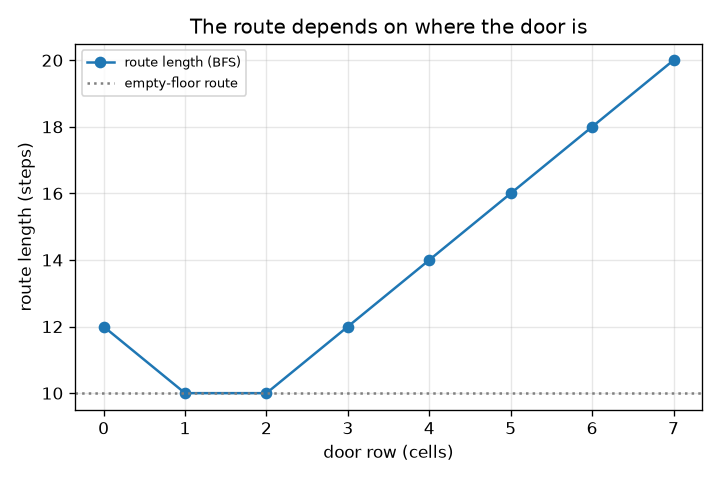
\includegraphics[width=0.85\linewidth]{figures/s01_route_vs_door.png}\\\small Route length against door row: best at rows 1 and 2 (10 steps), worst at row 7 (20 steps).\end{center}

\subsection*{E. Worked example}
The door is in row 6 and the shelf is in row 2. Find the number of steps, the straight-line distance and the extra steps caused by the wall.
\begin{enumerate}[nosep]
\item The robot starts at column 1, row 1. The shelf is at column 10, row 2. The robot must cross from column 1 to column 10: 9 steps to the right.
\item To pass the wall it must stand in row 6: from row 1 down to row 6 is \textbar{}1 - 6\textbar{} = 5 steps.
\item After the door it must go from row 6 to the shelf row 2: \textbar{}6 - 2\textbar{} = 4 steps.
\item Total = 9 + 5 + 4 = 18 steps. BFS in the checkpoint also returns 18.
\item Straight line = sqrt(9\textasciicircum{}2 + 1\textasciicircum{}2) = sqrt(82) = 9.06 cells. On an empty floor the route would be 9 + 1 = 10 steps, so the wall costs 8 extra steps.
\end{enumerate}
\textbf{Answer.} The route has 18 steps; the straight line is 9.06 cells; the wall adds 8 steps.

\subsection*{F. Questions}
\begin{enumerate}[nosep]
\item \textbf{Conceptual.} Why is the shortest route to the shelf longer than the straight line, and why can BFS stop as soon as it reaches the shelf?
\item \textbf{Numerical.} The door is in row 4 and the shelf is in row 2. How many steps is the route, and what is the straight-line distance? Check that the route is not shorter than the straight line.
\item \textbf{Graph and simulation interpretation.} In the graph of route length against door row (shelf in row 2), which door rows give the shortest route, what is that length, and why is it not smaller?
\item \textbf{Design and optimisation challenge.} Design: two kinds of orders go to shelves in row 2 and row 6, equally often. Choose the door row that minimises the total steps of one trip to each shelf. What is the total? What real-world factor does this model ignore that might change your choice?
\end{enumerate}

\section{Session 2: Graphs, Dijkstra and A*}

\subsection*{A. Real-world problem}
Real warehouse robots can move diagonally, and a diagonal move is longer than a straight one (sqrt 2 times). So 'fewest steps' is no longer 'cheapest route'. Also, a robot that thinks for a long time wastes time and battery, so we care about how many cells the search looks at. How wide should the aisles of a new warehouse be if we want many shelves but short routes? (Simplified model; not for real robot control.)

\subsection*{B. Concept and theory}
A node is a free cell. An edge joins neighbouring cells. In 4-connection a move up, down, left or right costs 1. In 8-connection the four diagonal moves cost sqrt 2 = 1.414; a diagonal may not cut a corner, so both cells beside it must be free. BFS minimises the number of moves; it is correct for cost only when all edges cost the same. Dijkstra keeps a priority queue (heapq) ordered by g, the cheapest known cost from the start, and always finishes the cheapest waiting node, so the first time it finishes the goal the cost is minimal. A* orders the queue by f = g + h, where h(n) estimates the cost still to go. If h never overestimates the true remaining cost (h is admissible), A* still returns the cheapest path: when the goal is finished with cost C, every node n on a truly cheaper path would have f(n) = g(n) + h(n) \textless{}= its true total cost \textless{} C, so it would have been finished earlier. A good h focuses the search toward the goal, so fewer nodes are expanded. Manhattan distance dx + dy is admissible on a 4-connected grid; octile distance (dx + dy) + (sqrt 2 - 2) min(dx, dy) is admissible (it is exact on an empty floor) on an 8-connected grid. Expanded nodes means nodes taken from the queue and finished; it is our measure of work.

\begin{itemize}[nosep]
\item g(n): cheapest known cost from the start to node n (cell widths)
\item h(n): estimated cost from n to the goal (cell widths)
\item f(n): g(n) + h(n), the queue priority (cell widths)
\item dx, dy: columns and rows between n and the goal (cells)
\item w: weight multiplying h (w = 1 is the normal A*) (no unit)
\end{itemize}

\begin{equation*}
f(n)=g(n)+h(n)
\end{equation*}

\begin{equation*}
h_{\mathrm{Manhattan}}=dx+dy
\end{equation*}

\begin{equation*}
h_{\mathrm{octile}}=(dx+dy)+(\sqrt2-2)\min(dx,dy)
\end{equation*}

\begin{equation*}
h(n)\le h^*(n)\ \text{for every }n\ \Rightarrow\ \text{A* returns a cheapest path}
\end{equation*}

\begin{center}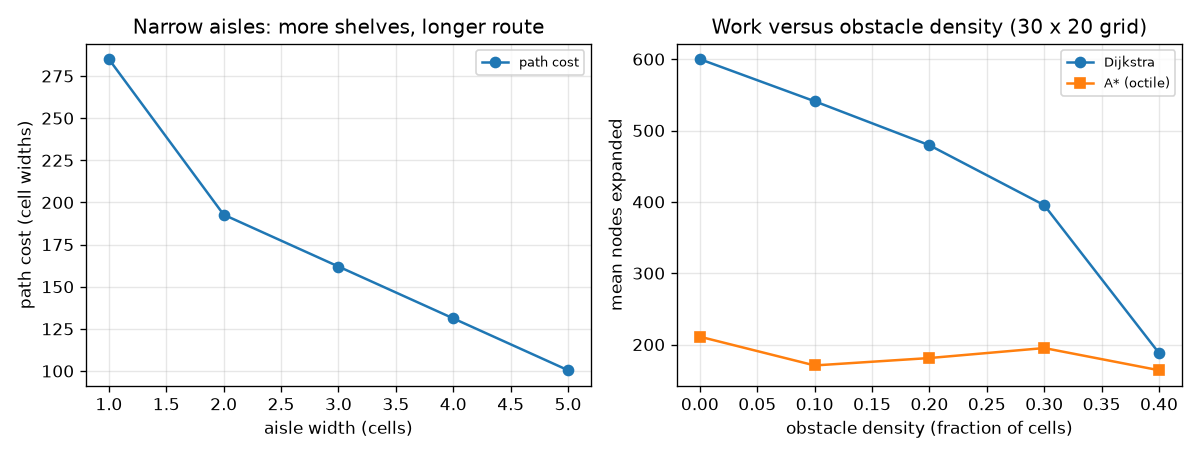
\includegraphics[width=0.85\linewidth]{figures/s02_aisle_density.png}\\\small Left: path cost against aisle width. Right: mean expanded nodes against obstacle density.\end{center}

\subsection*{E. Worked example}
On the 5 by 3 grid with a wall in column 2 (gap only in the bottom row), the robot at (0, 0) must reach (4, 1). Find the cheapest cost with 4 moves and with 8 moves, and compare with the Manhattan lower bound.
\begin{enumerate}[nosep]
\item Grid rows: 'S.\#..', '..\#.G', '.....'. Only row 2 passes the wall at column 2.
\item Manhattan distance from (0, 0) to (4, 1) is 4 + 1 = 5. This is a lower bound for 4 moves.
\item 4 moves: go down 2 rows to (0, 2), right 4 to (4, 2), up 1 to (4, 1): 2 + 4 + 1 = 7. The wall adds 2.
\item 8 moves: (0, 0) down to (0, 1) costs 1, diagonal to (1, 2) costs sqrt 2, right to (2, 2) and (3, 2) cost 1 + 1, diagonal up to (4, 1) costs sqrt 2 (both cells beside it are free).
\item Total = 1 + sqrt 2 + 1 + 1 + sqrt 2 = 3 + 2 sqrt 2 = 5.828. The diagonal from (1, 1) to (2, 2) is not allowed because (2, 1) is a wall.
\end{enumerate}
\textbf{Answer.} Cost 7 with 4 moves (above the Manhattan bound 5) and 3 + 2 sqrt 2 = 5.828 with 8 moves. BFS, Dijkstra and A* agree on these values.

\subsection*{F. Questions}
\begin{enumerate}[nosep]
\item \textbf{Conceptual.} Why does an admissible heuristic keep A* optimal, and what goes wrong if h overestimates?
\item \textbf{Numerical.} For a goal dx = 3 columns and dy = 1 row away on an empty 8-connected floor, compute the Manhattan, octile and straight-line distances and say which are admissible.
\item \textbf{Graph and simulation interpretation.} In the density graph, how does the work of Dijkstra change as the density of obstacles grows, and why does A* expand fewer nodes at every density?
\item \textbf{Design and optimisation challenge.} Design: in the 30 by 25 serpentine warehouse you need at least 200 shelf cells and a path cost of at most 170. Which aisle width (1 to 5 cells) do you choose, and what is the trade-off?
\end{enumerate}

\section{Session 3: Continuous space: RRT, RRT* and validation}

\subsection*{A. Real-world problem}
A grid forces the robot to move in eight directions and costs memory when the map is large and detailed. In continuous space a planner can use any direction, but we cannot list all positions. Sampling-based planners such as RRT (rapidly-exploring random tree) throw random points on the map and grow a tree of free moves. They are fast, but is the path good, and does the planner always find one? We answer with measurements against an exact answer. This is a simplified teaching model, not for controlling real robots or vehicles.

\subsection*{B. Concept and theory}
Obstacles are circles (centre, radius) and rectangles. A segment collides with a circle if its closest point to the centre is nearer than the radius. A segment collides with a rectangle if, after clipping it to the four sides (Liang-Barsky), a piece is left whose midpoint is strictly inside; touching an edge or a corner is allowed, because the shortest path around a wall must touch the wall corners. RRT repeats: sample a random point (with probability 0.05 the goal itself), find the nearest tree node, step from it toward the sample by at most the step size, and add the new node if that short segment is free. It stops when the goal is visible from the new node. RRT is probabilistically complete: if a path exists, the chance of finding it tends to 1 as iterations grow, but it does not promise the shortest path, and narrow passages need many samples. Shortcutting picks two points of the path and replaces everything between them by a straight segment if it is free. RRT* chooses as parent the nearby node that gives the lowest cost-from-start and rewires neighbours through the new node when that is cheaper, so its best path improves toward the optimum as iterations grow. Around a single wall the optimum is a polyline through the two top corners of the wall. Grid A* is optimal on the grid it is given, but the grid forces 8 directions; neither A* nor RRT gives both optimality and freedom from the grid for free.

\begin{itemize}[nosep]
\item step: largest distance the tree grows per iteration (m)
\item radius: neighbourhood size for RRT* parent choice and rewiring (m)
\item cost(n): length of the tree path from the start to node n (m)
\item t, h: wall thickness and wall height (m)
\item res: grid cell size for grid A* (m)
\end{itemize}

\begin{equation*}
\text{closest point on segment: } t^*=\mathrm{clip}\!\left(\frac{(c-p)\cdot(q-p)}{|q-p|^2},0,1\right),\quad \text{hit if } |p+t^*(q-p)-c|<r
\end{equation*}

\begin{equation*}
\text{exact wall path: } L=2\sqrt{(x_0-x_s)^2+(h-y_s)^2}+t\quad (x_0=5-t/2)
\end{equation*}

\begin{equation*}
\text{RRT* parent: } \arg\min_{j\in \mathrm{near}}\ \mathrm{cost}(j)+|x_j-x_{\mathrm{new}}|
\end{equation*}

\begin{center}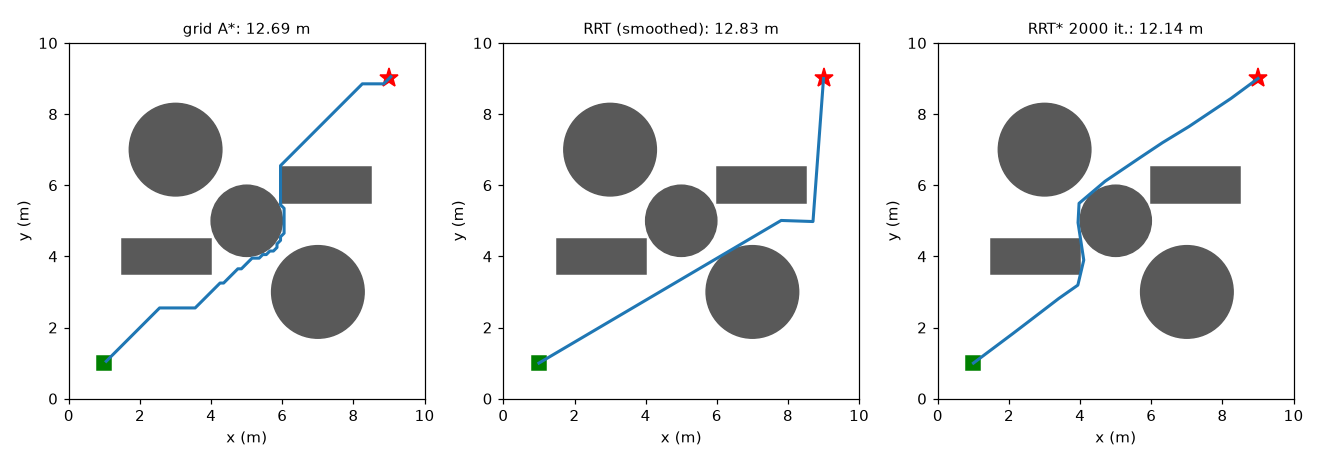
\includegraphics[width=0.85\linewidth]{figures/s03_planner_compare.png}\\\small Grid A*, smoothed RRT and RRT* on the same map.\end{center}

\subsection*{E. Worked example}
A thin wall (x from 4.8 to 5.2) rises from below the map to a height of 6 m. The robot starts at (1, 1) and the goal is at (9, 1). Find the exact shortest path and compare it with the straight line.
\begin{enumerate}[nosep]
\item The shortest path over the top is a polyline: start, left top corner (4.8, 6), right top corner (5.2, 6), goal.
\item First leg: dx = 4.8 - 1 = 3.8 and dy = 6 - 1 = 5, so length = sqrt(3.8\textasciicircum{}2 + 5\textasciicircum{}2) = sqrt(39.44) = 6.280 m.
\item Last leg is the mirror image: 6.280 m. The segment between the corners is 5.2 - 4.8 = 0.4 m.
\item Total = 2 * 6.280 + 0.4 = 12.960 m. A visibility-graph Dijkstra in the checkpoint finds the same polyline and length.
\item The straight line is 8 m, so the wall adds 4.960 m. Grid A* with 0.1 m cells returns 13.607 m (5 percent above), and RRT* after 3000 iterations returns 13.158 m (1.5 percent above).
\end{enumerate}
\textbf{Answer.} The exact shortest path is 12.960 m, through the two top corners of the wall; the straight line, 8 m, is blocked.

\subsection*{F. Questions}
\begin{enumerate}[nosep]
\item \textbf{Conceptual.} RRT is probabilistically complete but not optimal; A* is optimal on the grid. Explain what each statement means and why neither planner gives both properties for free.
\item \textbf{Numerical.} A thin wall (x from 4.8 to 5.2, height 6 m) has the start at (1, 3) and goal at (9, 3). Compute the exact shortest path length. Check it against the 8 m straight line.
\item \textbf{Graph and simulation interpretation.} From the RRT* cost graph, what happens to the best path length between 500 and 3000 iterations, and can it ever go below the red dashed line?
\item \textbf{Design and optimisation challenge.} Design: the narrow-passage map has a wall with a gap. Over 100 seeds with 1000 iterations and step 0.5 m, RRT succeeds 12 times for a 0.05 m gap, 33 for 0.1 m, 82 for 0.3 m and 100 for 1 m. A robot needs a gap of at least 0.3 m anyway. Which settings would you choose and what does the failure rate tell you about trusting RRT?
\end{enumerate}

\section{Real-world mini-project}
\textbf{Plan the pick route for a warehouse robot.} A 36 by 18 cell warehouse has nine shelf blocks, a dock at (1, 16) and four pick points at (6, 5), (21, 9), (31, 5) and (12, 13), to be visited in this order before returning to the dock. Each cell is 1 m wide (a simplifying assumption). Use \texttt{warehouse\_grid}, \texttt{DOCK}, \texttt{PICKS} and \texttt{pick\_route} from Session 3. Report the total route length and the number of nodes A* expanded, then repeat with Dijkstra (call \texttt{astar\_cells} with weight=0.0 for each leg) and compare the work.

\section{The path ahead}
\begin{enumerate}[nosep]
\item \textbf{Session 4: Choose the pick order.} A planner that reorders the four picks (then ten picks with a heuristic) before running A* between them.
\item \textbf{Session 5: Keep a safe distance.} Inflated obstacles and a path-clearance function, used by both grid A* and RRT*.
\item \textbf{Session 6: Find the narrow passage.} An RRT variant that samples more near obstacle edges.
\item \textbf{Session 7: Replan when an aisle is blocked.} A replanner that updates its route when one aisle cell becomes blocked.
\item \textbf{Session 8: Drivable paths for a car-like robot.} A planner whose paths have bounded curvature.
\end{enumerate}

\section{Answers and hints}

\subsection*{Session 1}
\begin{enumerate}[nosep]
\item \textbf{Conceptual.} Hint: Think about what the wall blocks, and about the order in which BFS visits cells. Solution: The straight line passes through blocked cells, so the robot cannot follow it; any allowed route must bend through the door, so it is longer. BFS visits all cells one step away before any cell two steps away, and so on, so the first time it reaches the shelf it has used the fewest possible steps. No later visit can be shorter.
\item \textbf{Numerical.} Hint: Use steps = 9 + \textbar{}1 - d\textbar{} + \textbar{}d - s\textbar{}. Solution: steps = 9 + \textbar{}1 - 4\textbar{} + \textbar{}4 - 2\textbar{} = 9 + 3 + 2 = 14 steps. Straight line = sqrt(82) = 9.06 cells. 14 is larger than 9.06, as it must be. Units: steps of one cell.
\item \textbf{Graph and simulation interpretation.} Hint: Find the lowest points and compare with the empty-floor line. Solution: Door rows 1 and 2 give 10 steps. 10 = 9 + 1 is the empty-floor value (9 columns and 1 row), so no wall position can do better: a wall can only add steps. Rows 0 and 3 give 12 steps, and row 7 gives 20.
\item \textbf{Design and optimisation challenge.} Hint: Add the two formulas for each door row 0 to 7 and compare. Solution: Totals for door rows 0 to 7 are 28, 24, 24, 26, 28, 30, 32, 36. Rows 1 and 2 tie with 24 steps. The model ignores congestion: if many robots use one door they queue, so a real design might add a second door. It also ignores door width and robot size.
\end{enumerate}

\subsection*{Session 2}
\begin{enumerate}[nosep]
\item \textbf{Conceptual.} Hint: Compare f = g + h of a node on the cheapest path with the cost of the path A* has already found. Solution: If h never overestimates, every node on a truly cheapest path has f at most the cheapest cost, so it is finished before any more expensive goal. If h overestimates, a node on the cheapest path can get an f above the cost of a worse path, so A* may finish the goal with the worse path first. In the lesson, multiplying the octile heuristic by 3 expands far fewer nodes but can return a longer path.
\item \textbf{Numerical.} Hint: Octile = (dx + dy) + (sqrt 2 - 2) min(dx, dy). Solution: Manhattan = 4. Octile = 4 + (1.414 - 2) * 1 = 3.414 (this is 2 + sqrt 2, which is also the true cost: two straight moves and one diagonal). Straight line = sqrt(10) = 3.162. On an 8-connected grid Manhattan (4) is larger than the true cost 3.414, so it is NOT admissible; octile and straight line are admissible (the straight line is admissible but weaker, so it focuses the search less).
\item \textbf{Graph and simulation interpretation.} Hint: Look at the two curves and think about what the heuristic knows. Solution: Dijkstra's mean expanded nodes fall as density grows (from 600 with no obstacles to 188 at density 0.4) because only grids where a path exists are counted and the obstacles block the flood. A* expands fewer nodes at every density because its heuristic pulls the search toward the goal while Dijkstra expands everything closer than the goal in all directions.
\item \textbf{Design and optimisation challenge.} Hint: Read the shelf cells and path cost for each aisle width from the lesson output. Solution: Aisle width 1 gives 464 shelf cells but cost 285.00; width 2 gives 290 cells and 192.73; width 3 gives 232 cells and 161.97; width 4 gives 174 cells and 131.21; width 5 gives 116 cells and 100.46. Only width 3 has at least 200 cells and cost at most 170. Trade-off: narrower aisles store more but make routes longer and, in a real warehouse, make passing impossible for two robots; wider aisles are faster but store less.
\end{enumerate}

\subsection*{Session 3}
\begin{enumerate}[nosep]
\item \textbf{Conceptual.} Hint: Think about what a random tree does after it finds the goal, and about what a grid does to directions. Solution: Probabilistically complete: if a path exists, the probability that RRT finds one tends to 1 as iterations grow, but RRT stops at the first path it finds, which is typically wiggly. A* gives the cheapest path among the grid's moves, but the grid allows only eight directions (and needs memory for every cell), so its path can be longer than the best true path (13.607 m against 12.960 m on the wall map). RRT* adds optimality only in the limit of many iterations and costs more time per iteration.
\item \textbf{Numerical.} Hint: Use L = 2 sqrt((4.8 - 1)\textasciicircum{}2 + (6 - 3)\textasciicircum{}2) + 0.4. Solution: L = 2 sqrt(3.8\textasciicircum{}2 + 3\textasciicircum{}2) + 0.4 = 2 sqrt(14.44 + 9) + 0.4 = 2 * 4.841 + 0.4 = 10.083 m. It is longer than the straight line (8 m), as it must be.
\item \textbf{Graph and simulation interpretation.} Hint: Look at the trend and at what the red line is. Solution: The best length falls from 14.792 m to 13.158 m and never increases (rewiring only lowers costs). It can never go below the red line, because the red line, 12.960 m, is the exact shortest path; RRT* only approaches it.
\item \textbf{Design and optimisation challenge.} Hint: Compare success rates and think about how many seeds (retries) you can afford. Solution: A robot with a minimum 0.3 m gap still sees 18 failures in 100 runs at 1000 iterations, so give RRT more iterations (500 iterations gave 24 successes for a 0.1 m gap and 1000 gave 33) or retry with several seeds, and keep a fallback such as A* on a grid fine enough to see the gap. Trust: RRT can fail even when a path exists; a failure is not a proof that none exists.
\end{enumerate}

\section{How to join}
Read \texttt{CONTRIBUTING.md} in the repository, then pick an issue labelled \texttt{good first issue}. Repository: \url{https://github.com/KrunalPanchal1995/openpathplanner}

\end{document}
